% Options for packages loaded elsewhere
% Options for packages loaded elsewhere
\PassOptionsToPackage{unicode}{hyperref}
\PassOptionsToPackage{hyphens}{url}
\PassOptionsToPackage{dvipsnames,svgnames,x11names}{xcolor}
%
\documentclass[
  letterpaper,
  DIV=11,
  numbers=noendperiod]{scrartcl}
\usepackage{xcolor}
\usepackage{amsmath,amssymb}
\setcounter{secnumdepth}{-\maxdimen} % remove section numbering
\usepackage{iftex}
\ifPDFTeX
  \usepackage[T1]{fontenc}
  \usepackage[utf8]{inputenc}
  \usepackage{textcomp} % provide euro and other symbols
\else % if luatex or xetex
  \usepackage{unicode-math} % this also loads fontspec
  \defaultfontfeatures{Scale=MatchLowercase}
  \defaultfontfeatures[\rmfamily]{Ligatures=TeX,Scale=1}
\fi
\usepackage{lmodern}
\ifPDFTeX\else
  % xetex/luatex font selection
\fi
% Use upquote if available, for straight quotes in verbatim environments
\IfFileExists{upquote.sty}{\usepackage{upquote}}{}
\IfFileExists{microtype.sty}{% use microtype if available
  \usepackage[]{microtype}
  \UseMicrotypeSet[protrusion]{basicmath} % disable protrusion for tt fonts
}{}
\makeatletter
\@ifundefined{KOMAClassName}{% if non-KOMA class
  \IfFileExists{parskip.sty}{%
    \usepackage{parskip}
  }{% else
    \setlength{\parindent}{0pt}
    \setlength{\parskip}{6pt plus 2pt minus 1pt}}
}{% if KOMA class
  \KOMAoptions{parskip=half}}
\makeatother
% Make \paragraph and \subparagraph free-standing
\makeatletter
\ifx\paragraph\undefined\else
  \let\oldparagraph\paragraph
  \renewcommand{\paragraph}{
    \@ifstar
      \xxxParagraphStar
      \xxxParagraphNoStar
  }
  \newcommand{\xxxParagraphStar}[1]{\oldparagraph*{#1}\mbox{}}
  \newcommand{\xxxParagraphNoStar}[1]{\oldparagraph{#1}\mbox{}}
\fi
\ifx\subparagraph\undefined\else
  \let\oldsubparagraph\subparagraph
  \renewcommand{\subparagraph}{
    \@ifstar
      \xxxSubParagraphStar
      \xxxSubParagraphNoStar
  }
  \newcommand{\xxxSubParagraphStar}[1]{\oldsubparagraph*{#1}\mbox{}}
  \newcommand{\xxxSubParagraphNoStar}[1]{\oldsubparagraph{#1}\mbox{}}
\fi
\makeatother


\usepackage{longtable,booktabs,array}
\usepackage{calc} % for calculating minipage widths
% Correct order of tables after \paragraph or \subparagraph
\usepackage{etoolbox}
\makeatletter
\patchcmd\longtable{\par}{\if@noskipsec\mbox{}\fi\par}{}{}
\makeatother
% Allow footnotes in longtable head/foot
\IfFileExists{footnotehyper.sty}{\usepackage{footnotehyper}}{\usepackage{footnote}}
\makesavenoteenv{longtable}
\usepackage{graphicx}
\makeatletter
\newsavebox\pandoc@box
\newcommand*\pandocbounded[1]{% scales image to fit in text height/width
  \sbox\pandoc@box{#1}%
  \Gscale@div\@tempa{\textheight}{\dimexpr\ht\pandoc@box+\dp\pandoc@box\relax}%
  \Gscale@div\@tempb{\linewidth}{\wd\pandoc@box}%
  \ifdim\@tempb\p@<\@tempa\p@\let\@tempa\@tempb\fi% select the smaller of both
  \ifdim\@tempa\p@<\p@\scalebox{\@tempa}{\usebox\pandoc@box}%
  \else\usebox{\pandoc@box}%
  \fi%
}
% Set default figure placement to htbp
\def\fps@figure{htbp}
\makeatother





\setlength{\emergencystretch}{3em} % prevent overfull lines

\providecommand{\tightlist}{%
  \setlength{\itemsep}{0pt}\setlength{\parskip}{0pt}}



 


\usepackage{booktabs}
\usepackage{longtable}
\usepackage{array}
\usepackage{multirow}
\usepackage{wrapfig}
\usepackage{float}
\usepackage{colortbl}
\usepackage{pdflscape}
\usepackage{tabu}
\usepackage{threeparttable}
\usepackage{threeparttablex}
\usepackage[normalem]{ulem}
\usepackage{makecell}
\usepackage{xcolor}
\KOMAoption{captions}{tableheading}
\makeatletter
\@ifpackageloaded{caption}{}{\usepackage{caption}}
\AtBeginDocument{%
\ifdefined\contentsname
  \renewcommand*\contentsname{Table of contents}
\else
  \newcommand\contentsname{Table of contents}
\fi
\ifdefined\listfigurename
  \renewcommand*\listfigurename{List of Figures}
\else
  \newcommand\listfigurename{List of Figures}
\fi
\ifdefined\listtablename
  \renewcommand*\listtablename{List of Tables}
\else
  \newcommand\listtablename{List of Tables}
\fi
\ifdefined\figurename
  \renewcommand*\figurename{Figure}
\else
  \newcommand\figurename{Figure}
\fi
\ifdefined\tablename
  \renewcommand*\tablename{Table}
\else
  \newcommand\tablename{Table}
\fi
}
\@ifpackageloaded{float}{}{\usepackage{float}}
\floatstyle{ruled}
\@ifundefined{c@chapter}{\newfloat{codelisting}{h}{lop}}{\newfloat{codelisting}{h}{lop}[chapter]}
\floatname{codelisting}{Listing}
\newcommand*\listoflistings{\listof{codelisting}{List of Listings}}
\makeatother
\makeatletter
\makeatother
\makeatletter
\@ifpackageloaded{caption}{}{\usepackage{caption}}
\@ifpackageloaded{subcaption}{}{\usepackage{subcaption}}
\makeatother
\usepackage{bookmark}
\IfFileExists{xurl.sty}{\usepackage{xurl}}{} % add URL line breaks if available
\urlstyle{same}
\hypersetup{
  pdftitle={Deeper Dive into vH4 (quarto)},
  colorlinks=true,
  linkcolor={blue},
  filecolor={Maroon},
  citecolor={Blue},
  urlcolor={Blue},
  pdfcreator={LaTeX via pandoc}}


\title{Deeper Dive into vH4 (quarto)}
\author{}
\date{}
\begin{document}
\maketitle


\section{METHODLOGY}\label{methodlogy}

Data was prepared as described in the separate report, ``Source Data,
Cleaning, and Preparation.'' This model trained on the years 2006 to
2023 and tested on data from the year 2024.

A predictive model was trained with the package ``xgboost.''

A value for math grade was predicted, and evaluated with the root mean
square error, mean absolute error, and r-squared values.

These values were also combined into a binary categorization
(``high''/``low'' or ``success''/``fail'' or ``on track''/``at risk'')
using various thresholds or cut-offs. An optimum threshold or cut-off
was discovered with the highest Kappa value.

\section{DISCUSSION}\label{discussion}

The model attempts to take information available at the time of
admittance, skip over course selection as a black box process, ignore
concurrent data such as class details (time of morning or capacity), and
predict grade performance for first-time freshmen at the end of their
initial math course. This comparison of the model with the timeline of
the actual student experience is shown in Figure~\ref{fig-pipeline}.

With this minimalist data set, the model could predict grades in initial
math courses for first-time freshmen with an R-squared value of 0.28,
root mean square error of 1.01, and mean absolute error of 0.8.

The variables most important to the model were the high school GPA, the
ACT math test scores, and their derivative z-scores and combined z-score
distance to the qualifications of the prior year's median successful
student.

This aligns with a theory of performance\footnote{Anderson, N. H., \&
  Butzin, C. A. 1974. Performance = motivation X ability: An
  integration-theoretical analysis. Journal of Personality and Social
  Psychology, 30(5): 598--604. \url{https://doi.org/10.1037/h0037447}}
(Figure~\ref{fig-performance}) where a student's math ability (as
measured by the ACT math test scores) and a student's `study ability'
(as measured by their high school GPA) are strong predictors of
performance. However, the model is not completely determinative -- the
pre-University data doesn't define the grade received -- leaving room
for individual motivation, effort, and the influence of the concurrent
situation (such as the number of credits taken that semester). No
student is guaranteed an `A', as many students who are predicted to
score well do poorly (and vice versa.)

Given the sparsity of the data, the model tended to predict in the
middle of the range, putting 47\% of the students between a grade of 2.7
and 3.7, while some 39\% of students in 2024 actually received an `A'.
Several comparisons of the predicted and actual grades are presented as
scatter plots or box plots (Figure~\ref{fig-results_scatter_box}),
density plots (Figure~\ref{fig-density}), heat maps
(Figure~\ref{fig-heatmap}), confusion matrices
(Figure~\ref{fig-binary_cm}, Figure~\ref{fig-fail_cm}), and histograms
(Figure~\ref{fig-pred_hist_actual}, Figure~\ref{fig-pred_hist_predict}).

An optimum binary threshold was found at a predicted grade of 2.4, with
a Kappa value of 0.41. Students predicted to have a grade less than 2.4
are a high-risk group of students. 29\% of these 507 students actually
did fail, or 76\% of the total of students who failed. (76\% recall and
29\% precision).

This compares to the risk of students predicted to have a grade more
than 2.4. Only 47 of these 1195 students failed, or 4\%.

Only a handful of students were precisely predicted fail their initial
math course -- eight students were predicted to receive a grade less
than 0.9, and six of these students actually received a grade less than
0.9. These students might be considered admissions mistakes, as they
predictably failed. However, out of 1,759 students, this doesn't seem to
indicate a large problem with admissions standards.

\section{CONCLUSIONS}\label{conclusions}

The model could predict grades in initial math courses for first-time
freshmen with an R-squared value of 0.28, root mean square error of
1.01, and mean absolute error of 0.8. The variables most important to
the model were the high school GPA, the ACT math test scores, and their
derivative z-scores and combined distance.

The model had optimum performance in separating an at-risk population
and a successful population at a predicted grade threshold of 2.4
(between a C-plus and a B-minus.) Accuracy at this cut-off had a Kappa
value of 0.41.

At this cut-off, the actual failure metrics (grades less than a 1.7)
were 76\% recall and 29\% precision, or roughly one-third of the
identified ``at risk'' group actually failed and one out of twenty-five
of the ``successful'' group actually failed.

\section{POSSIBLE NEXT STEPS}\label{possible-next-steps}

Grade prediction accuracy should increase with the inclusion of
concurrent data, such as:

\begin{itemize}
\tightlist
\item
  The number of credits taken
\item
  Difficulty of concurrent classes
\item
  Initial course grades on quizzes, homework, and initial tests\\
\item
  Utilization of tutoring services\\
\item
  Participation in study groups
\end{itemize}

The model might improve with an indicator that clusters similar classes
(in terms of incoming qualifications) together. This could help
differentiate many small courses by combining them.

\section{RESULTS}\label{results}

\begin{figure}

\caption{\label{fig-pipeline}Model compared to the timeline of actual
student experience}

\centering{

\pandocbounded{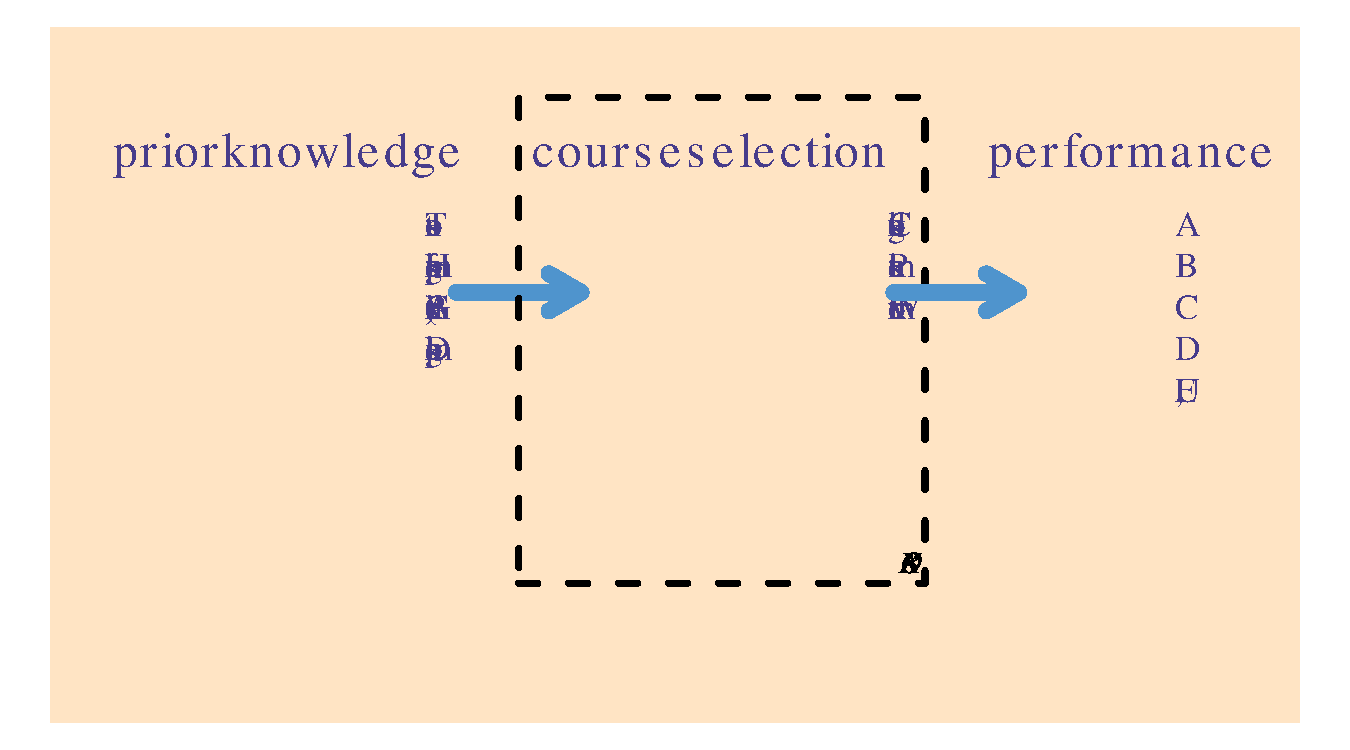
\includegraphics[keepaspectratio]{Deeper-Dive-into-vH4-model--quarto-_files/figure-pdf/fig-pipeline-1.pdf}}

}

\end{figure}%

\begin{table}

\caption{\label{tbl-results}Regression Results}

\centering{

\centering
\begin{tabular}[t]{cccccccc}
\toprule
\multicolumn{1}{c}{ } & \multicolumn{3}{c}{Raw Metrics} & \multicolumn{4}{c}{Normalized Metrics} \\
\cmidrule(l{3pt}r{3pt}){2-4} \cmidrule(l{3pt}r{3pt}){5-8}
 & RMSE & MAE & R-sq & NRMSE (Range) & NMAE (Range) & NRMSE (SD) & NMAE (SD)\\
\midrule
\cellcolor{gray!10}{GRADEGPA} & \cellcolor{gray!10}{1.01} & \cellcolor{gray!10}{0.8} & \cellcolor{gray!10}{0.28} & \cellcolor{gray!10}{0.25} & \cellcolor{gray!10}{0.2} & \cellcolor{gray!10}{0.89} & \cellcolor{gray!10}{0.7}\\
\bottomrule
\end{tabular}

}

\end{table}%

\begin{figure}

\caption{\label{fig-results_scatter_box}These plots show what the
correct prediction value would be with a red line.}

\centering{

\pandocbounded{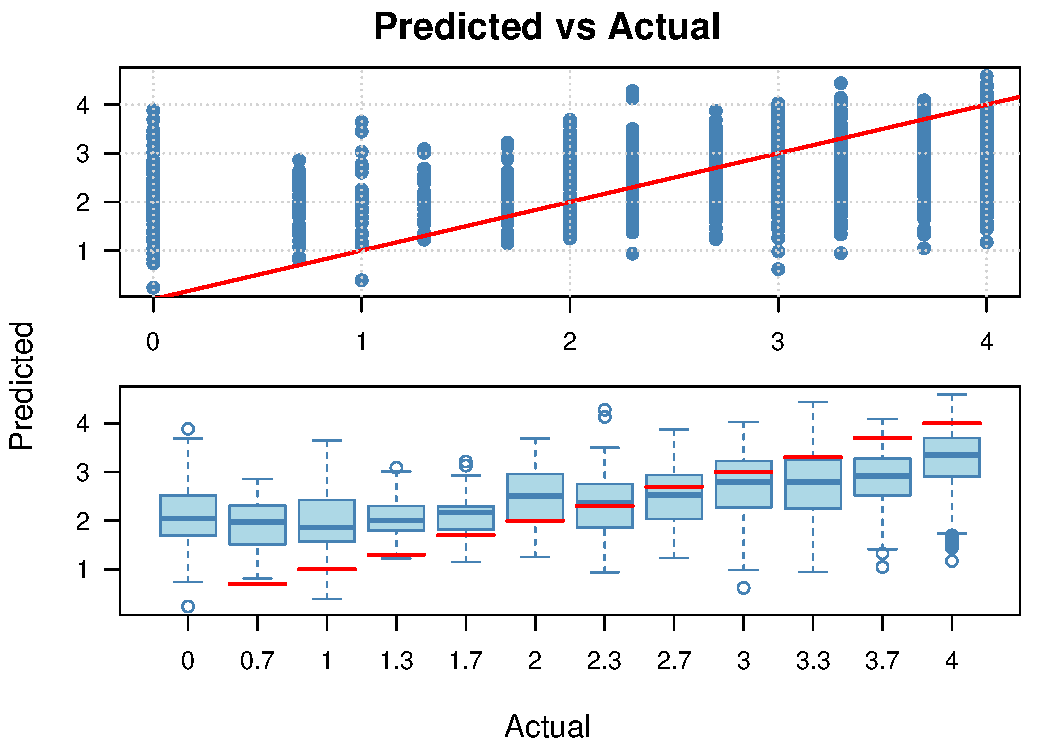
\includegraphics[keepaspectratio]{Deeper-Dive-into-vH4-model--quarto-_files/figure-pdf/fig-results_scatter_box-1.pdf}}

}

\end{figure}%

\begin{figure}

\caption{\label{fig-density}The model tends to predict towards the
center, while most students earn an `A'.}

\centering{

\pandocbounded{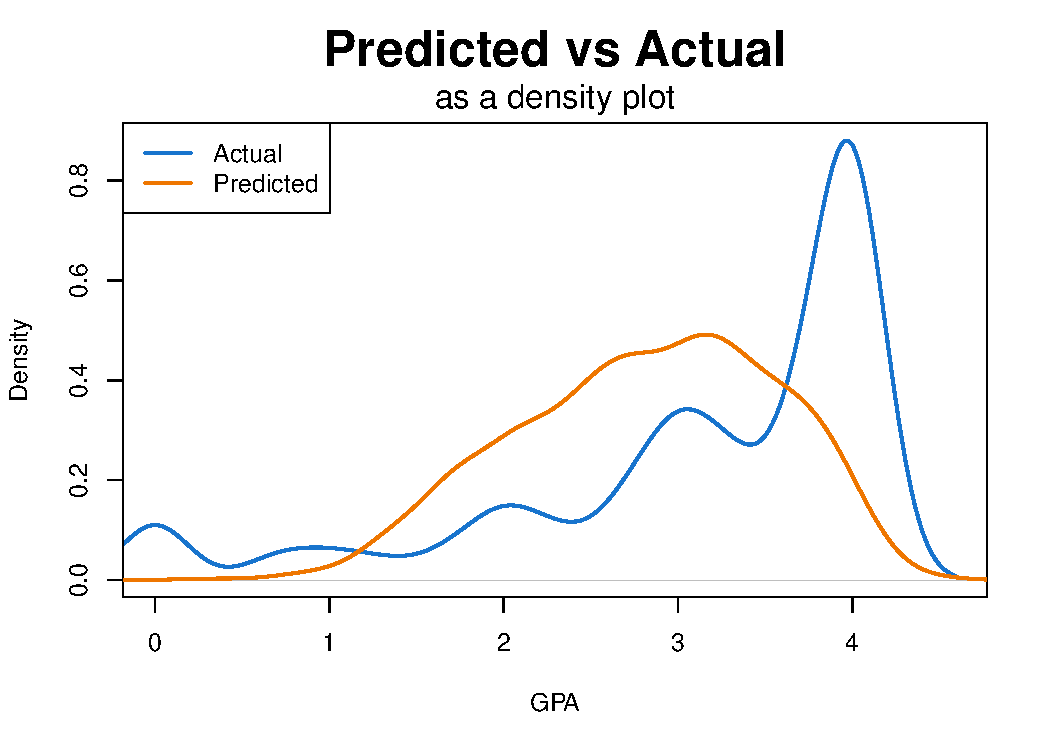
\includegraphics[keepaspectratio]{Deeper-Dive-into-vH4-model--quarto-_files/figure-pdf/fig-density-1.pdf}}

}

\end{figure}%

\begin{figure}

\caption{\label{fig-heatmap}The heatmap shows grade expectations
increase with ACT Math and high school GPA.}

\centering{

\pandocbounded{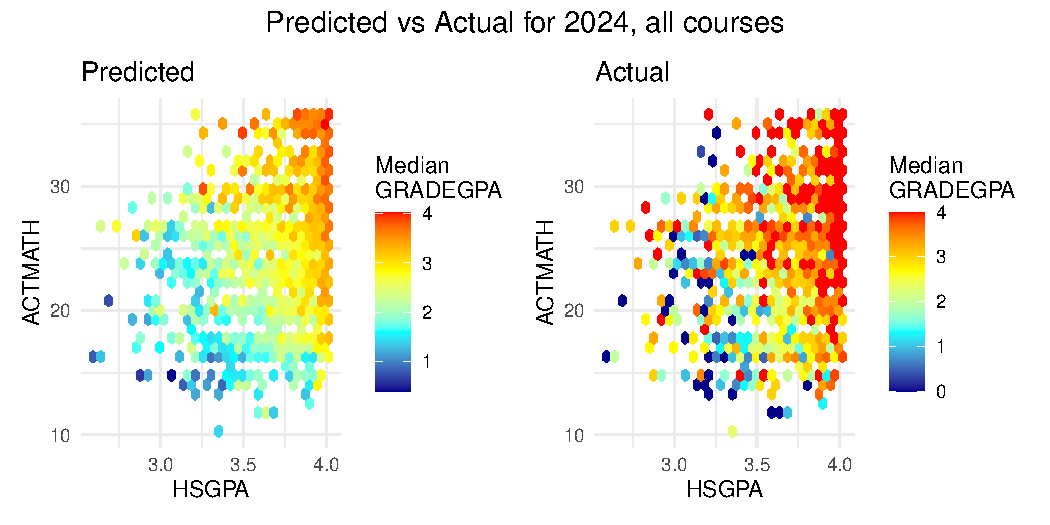
\includegraphics[keepaspectratio]{Deeper-Dive-into-vH4-model--quarto-_files/figure-pdf/fig-heatmap-1.pdf}}

}

\end{figure}%

\subsection{Selection of model optimum binary cut-off or
threshold}\label{selection-of-model-optimum-binary-cut-off-or-threshold}

The model has the highest accuracy in separating into high/low (or
succeed/at-risk) populations at a predicted grade of 2.4, between an
actual grade of C-plus (2.3) and B-minus (2.7).

\begin{figure}

\caption{\label{fig-threshold}Selection of model optimum cut-off}

\centering{

\pandocbounded{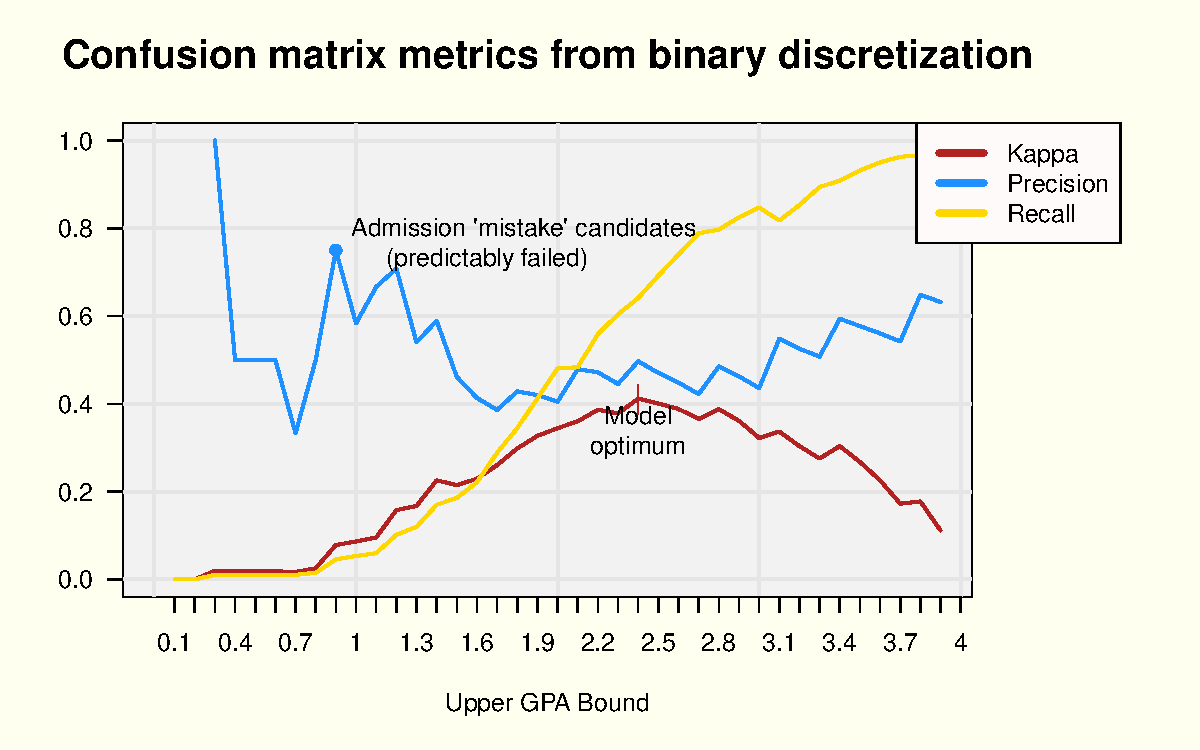
\includegraphics[keepaspectratio]{Deeper-Dive-into-vH4-model--quarto-_files/figure-pdf/fig-threshold-1.pdf}}

}

\end{figure}%

\begin{figure}

\caption{\label{fig-binary_cm}Confusion matrix at model binary optimum}

\centering{

\pandocbounded{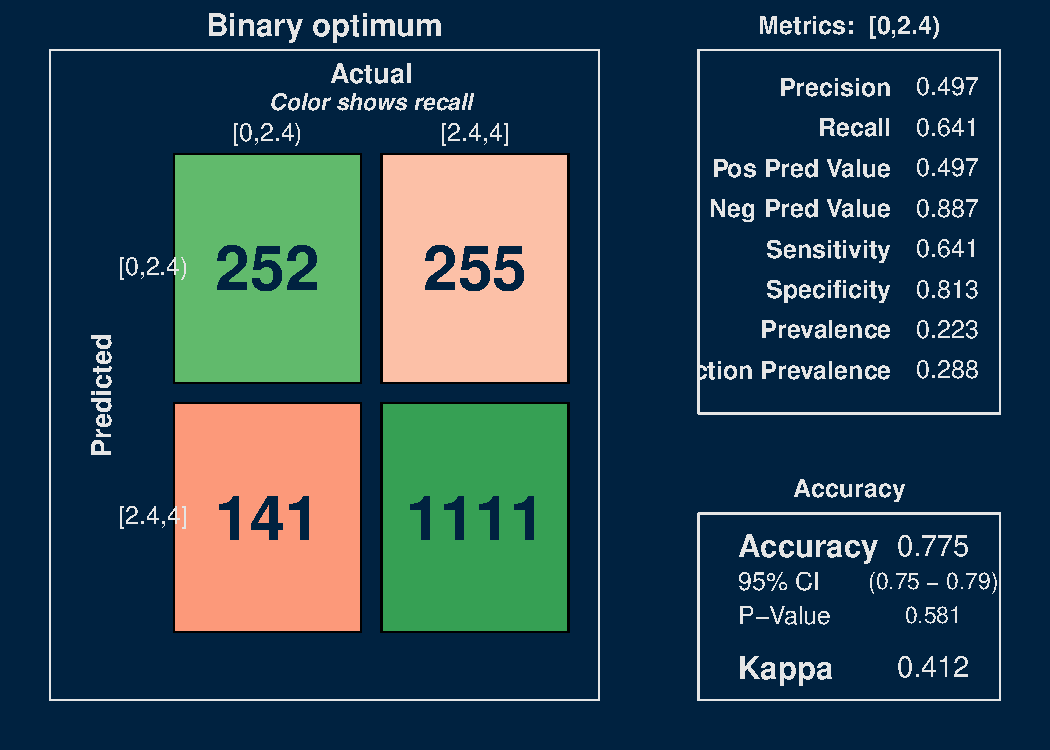
\includegraphics[keepaspectratio]{Deeper-Dive-into-vH4-model--quarto-_files/figure-pdf/fig-binary_cm-1.pdf}}

}

\end{figure}%

\begin{table}

\caption{\label{tbl-risk}Actual failure rates of `Success' and `At Risk'
populations at model binary optimum}

\centering{

\centering
\begin{tabular}[t]{ccc}
\toprule
\multicolumn{1}{c}{ } & \multicolumn{2}{c}{Actual Grade} \\
\cmidrule(l{3pt}r{3pt}){2-3}
\textbf{Predicted Grade} & \textbf{Actual: Fail (<1.7)} & \textbf{Actual: Pass (≥1.7)}\\
\midrule
{}[0,2.4] & 147
(8.6%) & 360
\cellcolor{gray!10}{(21.2%)}\\
(2.4,4] & 47
(2.8%) & 1148
(67.5%)\\
\bottomrule
\end{tabular}

}

\end{table}%

Students predicted to have a grade less than 2.4 are a high-risk group
of students. 29\% of these 507 students actually did fail, or 76\% of
the total of students who failed. (76\% recall and 29\% precision).

This compares to the risk of students predicted to have a grade more
than 2.4. Only 47 of these 1195 students failed, or 4\%.

The following histograms compare the ranges of grades predicted and
actually received. In Figure~\ref{fig-pred_hist_actual}, 69 students
predicted to get a grade less than 2.4 received a grade of zero. In
Figure~\ref{fig-pred_hist_predict}, of the students who actually
received a grade less than 2.4, only nine of them were predicted to get
a grade less than one.

\begin{figure}

\caption{\label{fig-pred_hist_actual}Illustration of prediction
accuracy: where the histogram shows the actual grades received for the
grades predicted in the dotted box.}

\centering{

\pandocbounded{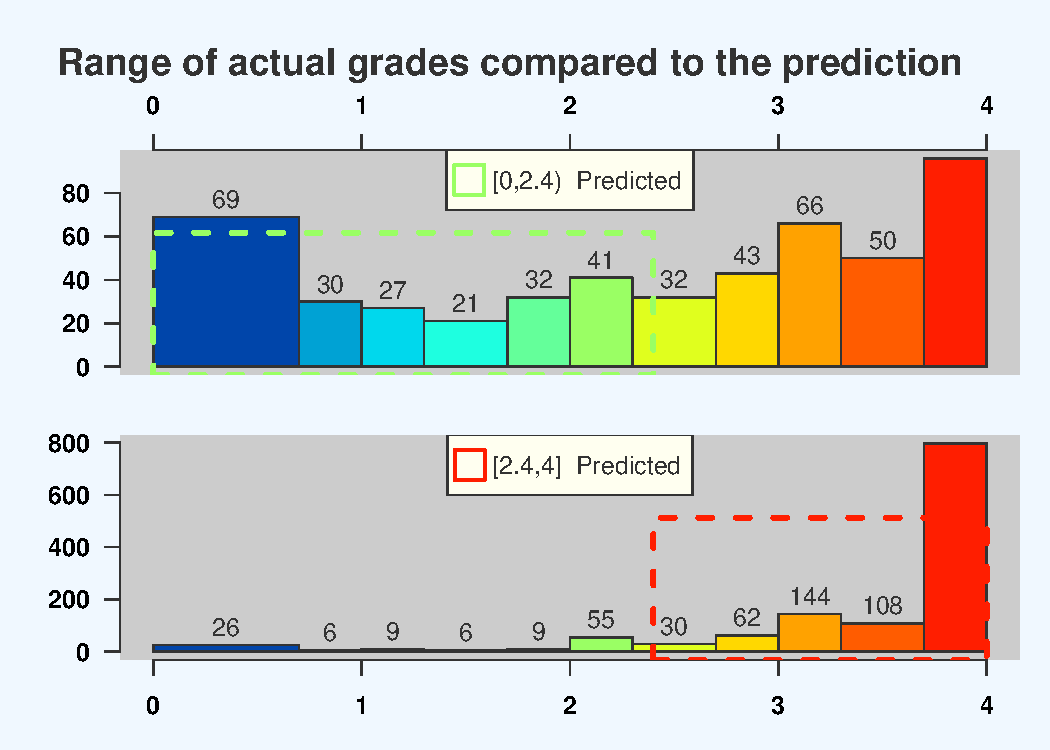
\includegraphics[keepaspectratio]{Deeper-Dive-into-vH4-model--quarto-_files/figure-pdf/fig-pred_hist_actual-1.pdf}}

}

\end{figure}%

\begin{figure}

\caption{\label{fig-pred_hist_predict}Illustration of prediction
accuracy: where the histogram shows the predicted grades for the actual
grades received in the dotted box.}

\centering{

\pandocbounded{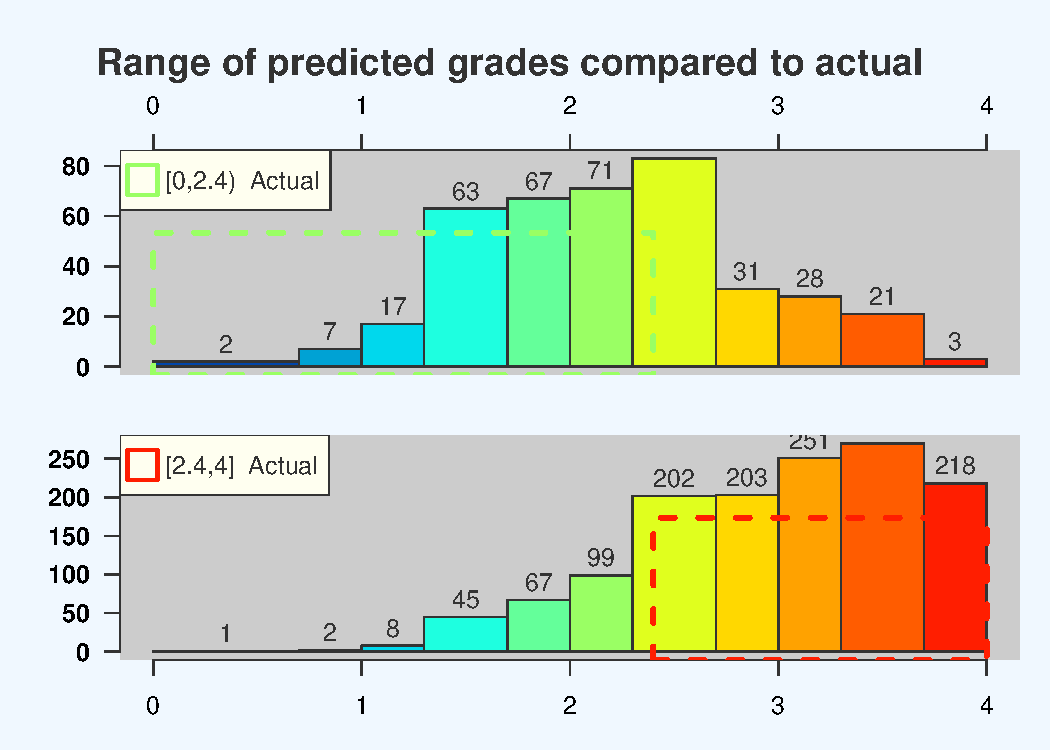
\includegraphics[keepaspectratio]{Deeper-Dive-into-vH4-model--quarto-_files/figure-pdf/fig-pred_hist_predict-1.pdf}}

}

\end{figure}%

This model also shows a high precision point at a predicted GPA of 0.9.
These candidates would predictably fail, and could be considered an
admissions mistake. However, there are only eight people so identified
(out of 1,759), suggesting nearly all students admitted to the U have a
strong expectation of passing initial math courses.

\begin{figure}

\caption{\label{fig-fail_cm}Confusion matrix for `admission mistake'
candidates}

\centering{

\pandocbounded{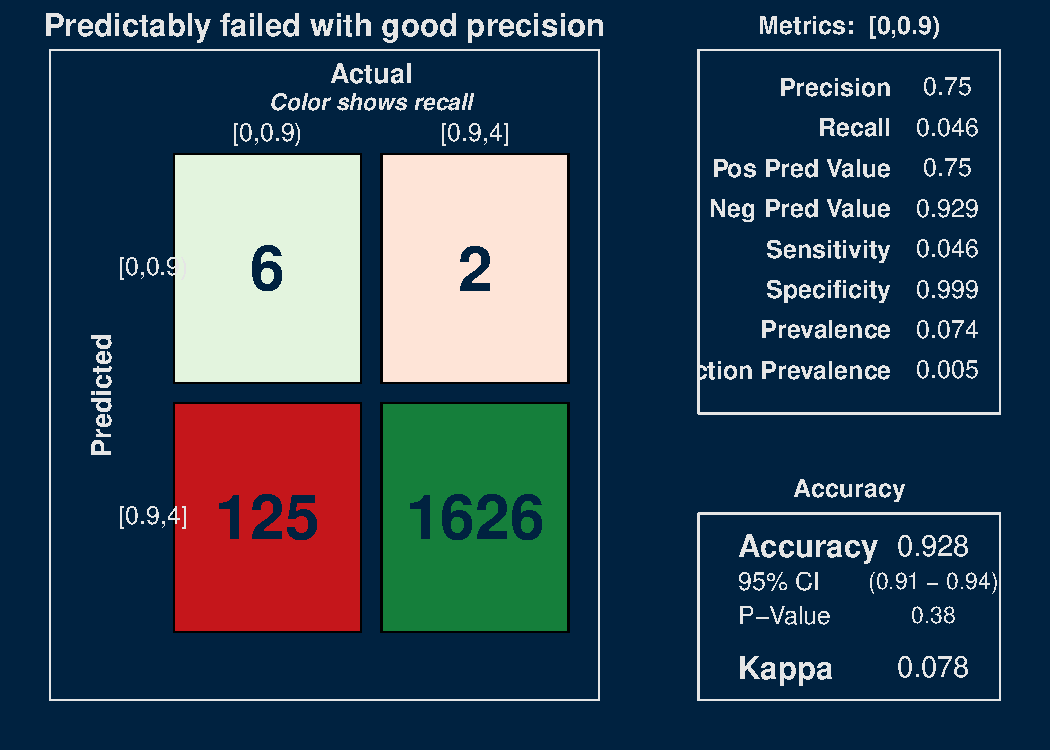
\includegraphics[keepaspectratio]{Deeper-Dive-into-vH4-model--quarto-_files/figure-pdf/fig-fail_cm-1.pdf}}

}

\end{figure}%

\subsection{Variable importance}\label{variable-importance}

\begin{figure}

\caption{\label{fig-importance}Variable importance to the model}

\centering{

\pandocbounded{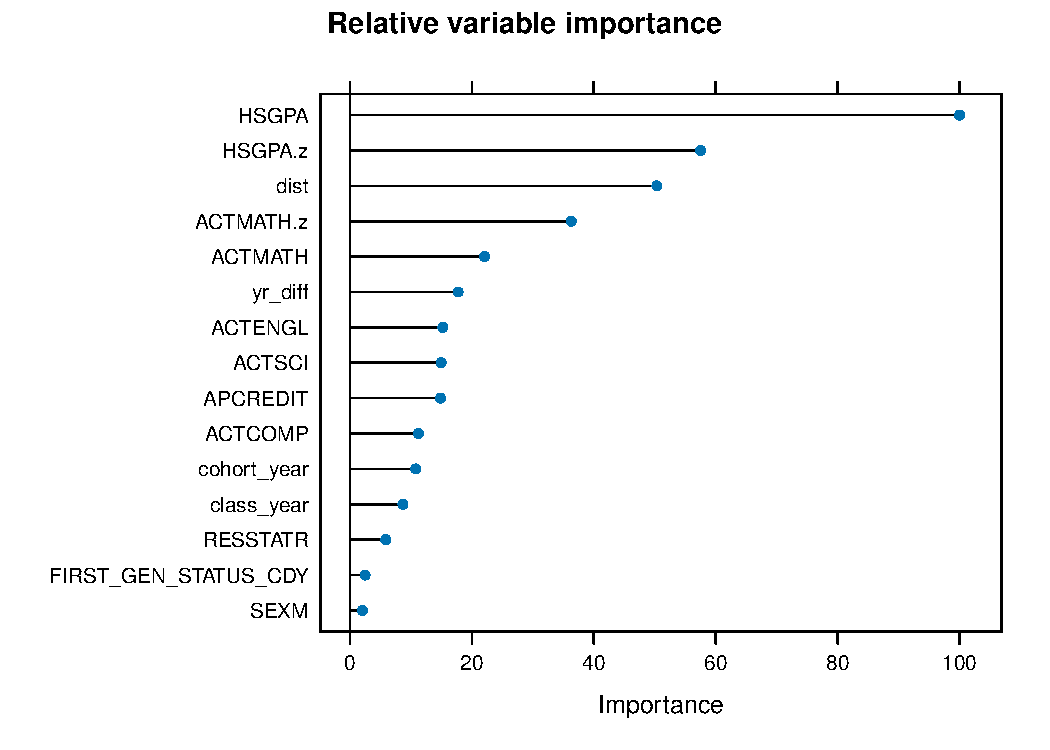
\includegraphics[keepaspectratio]{Deeper-Dive-into-vH4-model--quarto-_files/figure-pdf/fig-importance-1.pdf}}

}

\end{figure}%

\begin{figure}

\caption{\label{fig-performance}Theory of performance}

\centering{

\pandocbounded{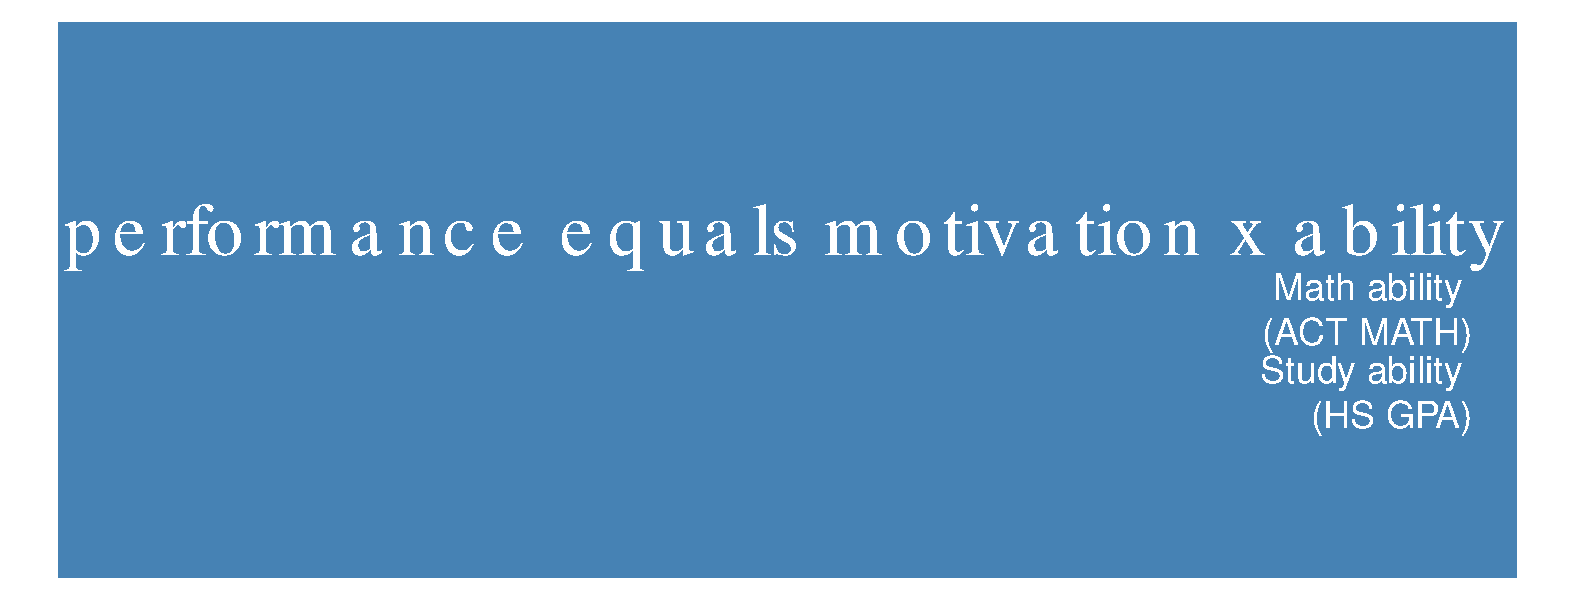
\includegraphics[keepaspectratio]{Deeper-Dive-into-vH4-model--quarto-_files/figure-pdf/fig-performance-1.pdf}}

}

\end{figure}%

\begin{figure}

\caption{\label{fig-gpa}\#1 Variable: High school GPA}

\centering{

\pandocbounded{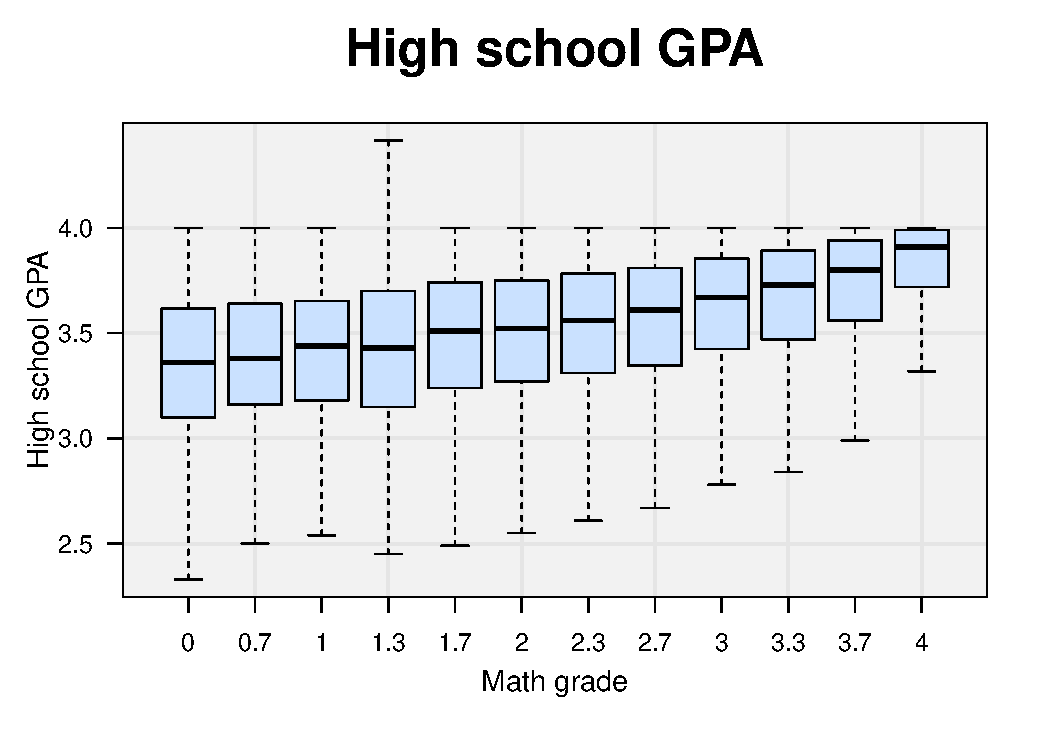
\includegraphics[keepaspectratio]{Deeper-Dive-into-vH4-model--quarto-_files/figure-pdf/fig-gpa-1.pdf}}

}

\end{figure}%

\begin{figure}

\caption{\label{fig-gpa_z}\#2 Variable: High school GPA z-score}

\centering{

\pandocbounded{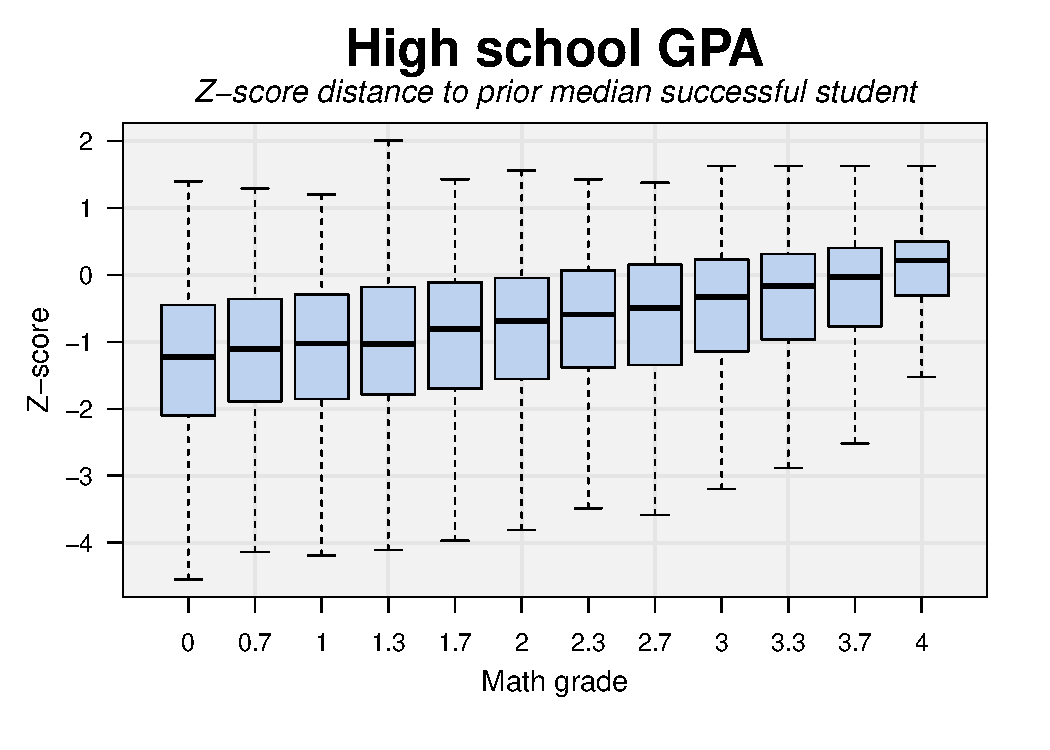
\includegraphics[keepaspectratio]{Deeper-Dive-into-vH4-model--quarto-_files/figure-pdf/fig-gpa_z-1.pdf}}

}

\end{figure}%

\begin{figure}

\caption{\label{fig-dist}\#3 Variable: Combined z-score distance}

\centering{

\pandocbounded{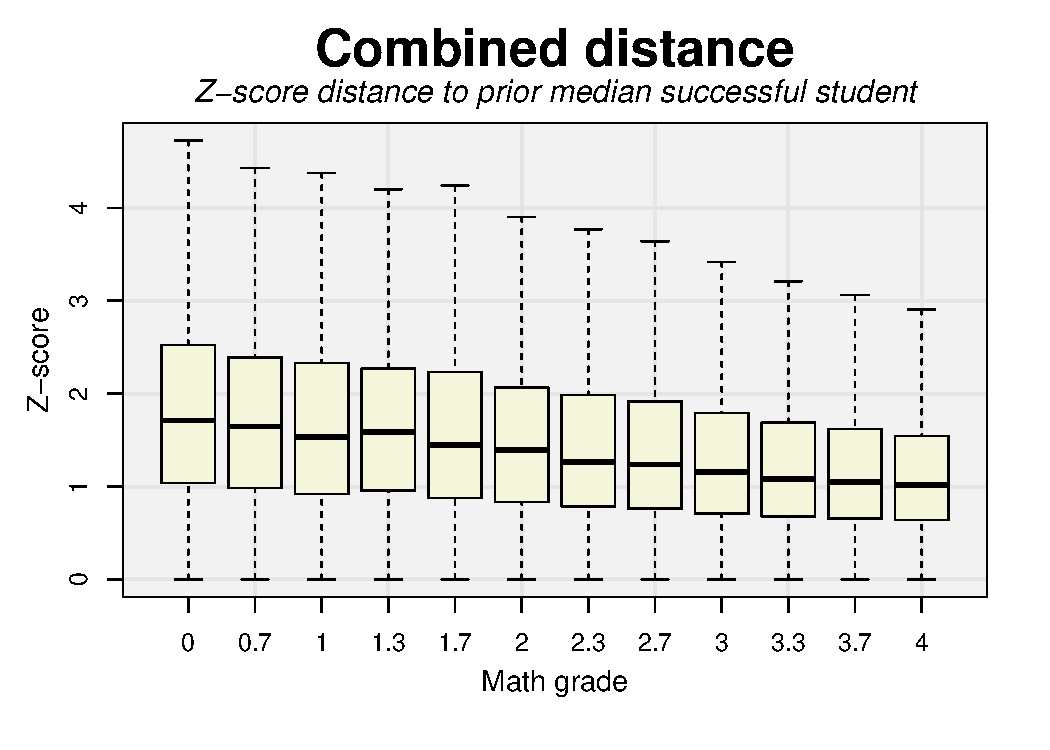
\includegraphics[keepaspectratio]{Deeper-Dive-into-vH4-model--quarto-_files/figure-pdf/fig-dist-1.pdf}}

}

\end{figure}%

\begin{figure}

\caption{\label{fig-act_z}\#4 Variable: ACT Math z-score}

\centering{

\pandocbounded{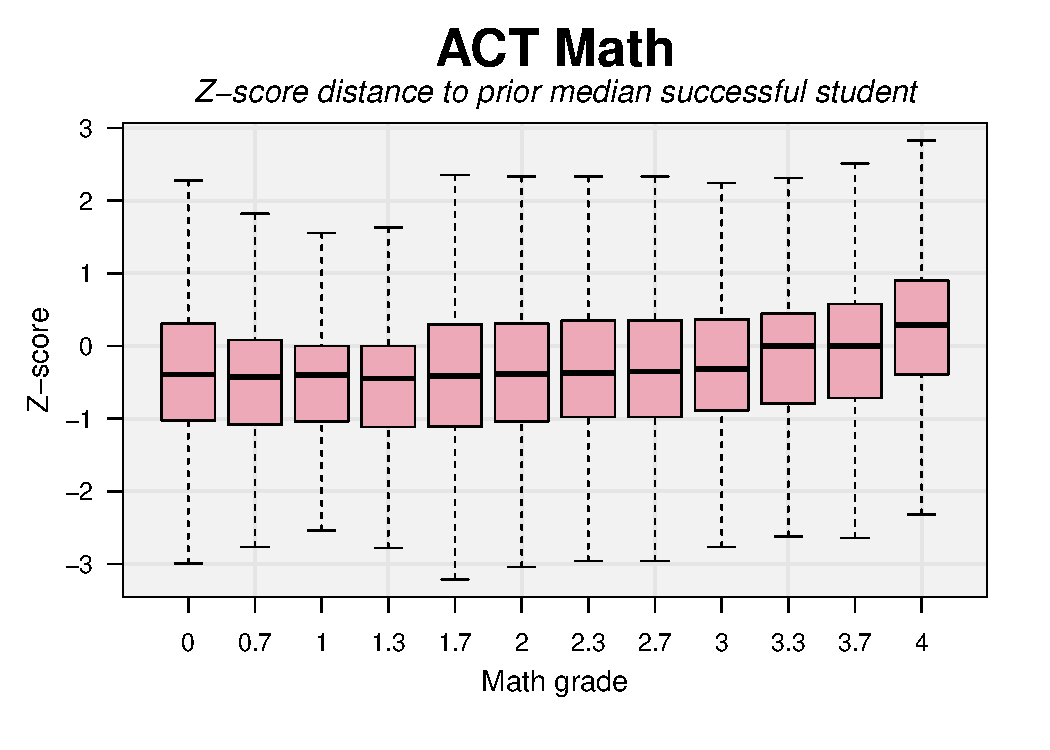
\includegraphics[keepaspectratio]{Deeper-Dive-into-vH4-model--quarto-_files/figure-pdf/fig-act_z-1.pdf}}

}

\end{figure}%

\begin{figure}

\caption{\label{fig-act}\#5 Variable: ACT Math}

\centering{

\pandocbounded{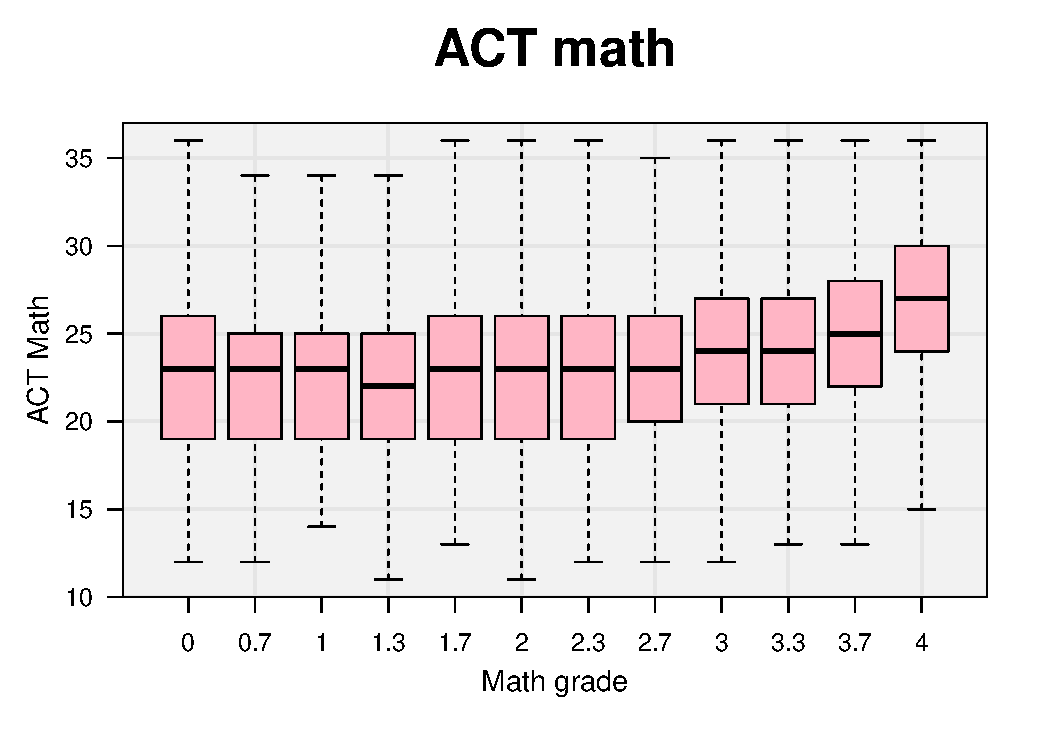
\includegraphics[keepaspectratio]{Deeper-Dive-into-vH4-model--quarto-_files/figure-pdf/fig-act-1.pdf}}

}

\end{figure}%

\begin{figure}

\caption{\label{fig-yr_diff}\#6 Variable: Years to initial math course}

\centering{

\pandocbounded{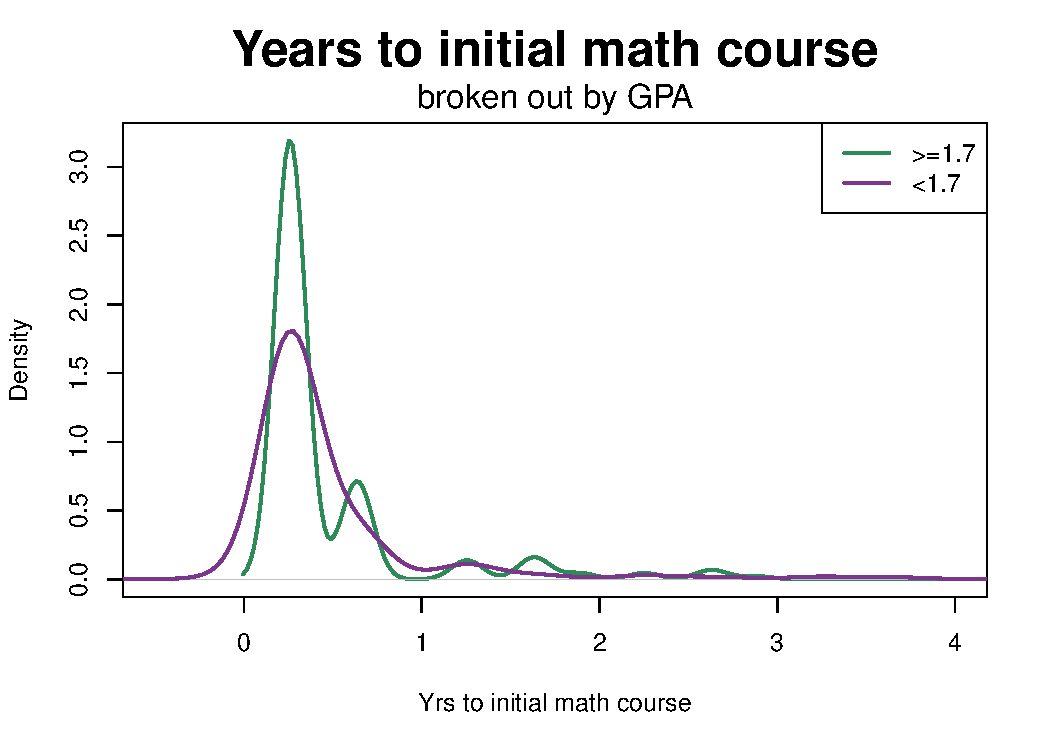
\includegraphics[keepaspectratio]{Deeper-Dive-into-vH4-model--quarto-_files/figure-pdf/fig-yr_diff-1.pdf}}

}

\end{figure}%

There is a small tendency for people who fail to take the initial math
course after the first year. (Most students (89\% in 2024) take their
initial math course in the first year.)

\section{REFERENCES}\label{references}

\begin{figure}

\caption{\label{fig-guide}How to interpret a confusion matrix}

\centering{

\pandocbounded{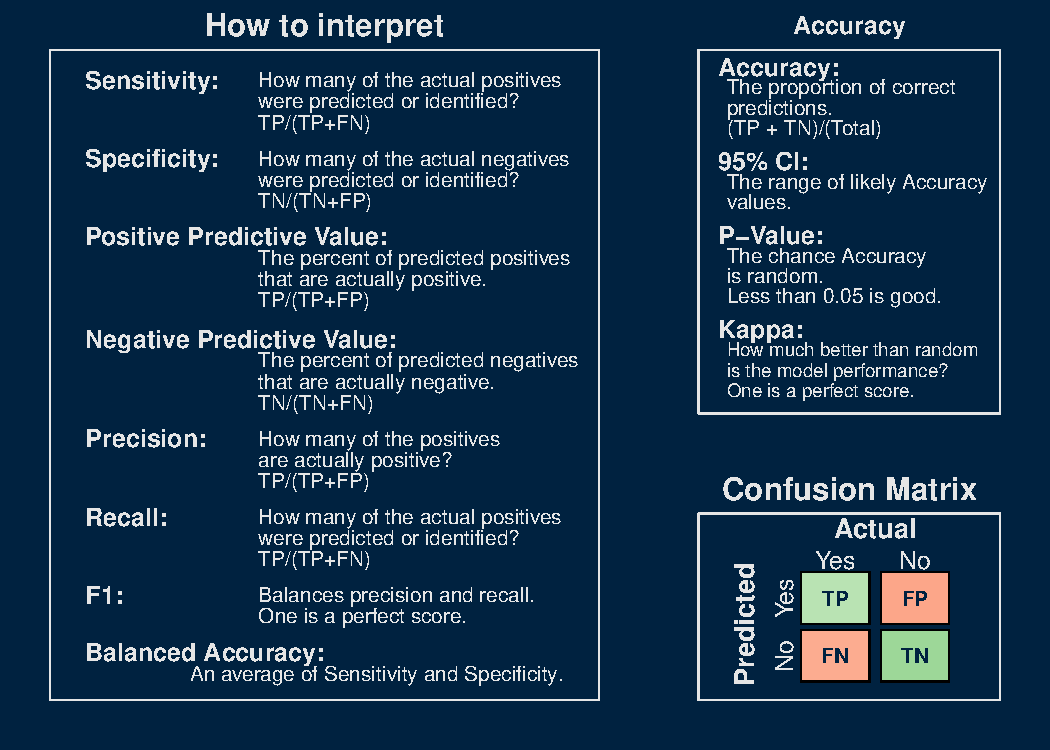
\includegraphics[keepaspectratio]{Deeper-Dive-into-vH4-model--quarto-_files/figure-pdf/fig-guide-1.pdf}}

}

\end{figure}%

\subsection{Training data}\label{training-data}

\begin{longtable}[]{@{}ll@{}}
\caption{Data summary}\tabularnewline
\toprule\noalign{}
\endfirsthead
\endhead
\bottomrule\noalign{}
\endlastfoot
Name & data\_list{[}{[}``GRADEGPA''{]}{]}{[}{[}\ldots{} \\
Number of rows & 36924 \\
Number of columns & 24 \\
\_\_\_\_\_\_\_\_\_\_\_\_\_\_\_\_\_\_\_\_\_\_\_ & \\
Column type frequency: & \\
character & 5 \\
factor & 3 \\
numeric & 16 \\
\_\_\_\_\_\_\_\_\_\_\_\_\_\_\_\_\_\_\_\_\_\_\_\_ & \\
Group variables & None \\
\end{longtable}

\textbf{Variable type: character}

\begin{longtable}[]{@{}
  >{\raggedright\arraybackslash}p{(\linewidth - 14\tabcolsep) * \real{0.2564}}
  >{\raggedleft\arraybackslash}p{(\linewidth - 14\tabcolsep) * \real{0.1282}}
  >{\raggedleft\arraybackslash}p{(\linewidth - 14\tabcolsep) * \real{0.1795}}
  >{\raggedleft\arraybackslash}p{(\linewidth - 14\tabcolsep) * \real{0.0513}}
  >{\raggedleft\arraybackslash}p{(\linewidth - 14\tabcolsep) * \real{0.0513}}
  >{\raggedleft\arraybackslash}p{(\linewidth - 14\tabcolsep) * \real{0.0769}}
  >{\raggedleft\arraybackslash}p{(\linewidth - 14\tabcolsep) * \real{0.1154}}
  >{\raggedleft\arraybackslash}p{(\linewidth - 14\tabcolsep) * \real{0.1410}}@{}}
\toprule\noalign{}
\begin{minipage}[b]{\linewidth}\raggedright
skim\_variable
\end{minipage} & \begin{minipage}[b]{\linewidth}\raggedleft
n\_missing
\end{minipage} & \begin{minipage}[b]{\linewidth}\raggedleft
complete\_rate
\end{minipage} & \begin{minipage}[b]{\linewidth}\raggedleft
min
\end{minipage} & \begin{minipage}[b]{\linewidth}\raggedleft
max
\end{minipage} & \begin{minipage}[b]{\linewidth}\raggedleft
empty
\end{minipage} & \begin{minipage}[b]{\linewidth}\raggedleft
n\_unique
\end{minipage} & \begin{minipage}[b]{\linewidth}\raggedleft
whitespace
\end{minipage} \\
\midrule\noalign{}
\endhead
\bottomrule\noalign{}
\endlastfoot
SEX & 0 & 1 & 1 & 1 & 0 & 2 & 0 \\
FIRST\_GEN\_STATUS\_CD & 0 & 1 & 1 & 1 & 0 & 3 & 0 \\
RESSTAT & 0 & 1 & 1 & 1 & 0 & 2 & 0 \\
HSPRIVATE & 0 & 1 & 1 & 1 & 0 & 2 & 0 \\
season & 0 & 1 & 4 & 6 & 0 & 3 & 0 \\
\end{longtable}

\textbf{Variable type: factor}

\begin{longtable}[]{@{}
  >{\raggedright\arraybackslash}p{(\linewidth - 10\tabcolsep) * \real{0.1414}}
  >{\raggedleft\arraybackslash}p{(\linewidth - 10\tabcolsep) * \real{0.1010}}
  >{\raggedleft\arraybackslash}p{(\linewidth - 10\tabcolsep) * \real{0.1414}}
  >{\raggedright\arraybackslash}p{(\linewidth - 10\tabcolsep) * \real{0.0808}}
  >{\raggedleft\arraybackslash}p{(\linewidth - 10\tabcolsep) * \real{0.0909}}
  >{\raggedright\arraybackslash}p{(\linewidth - 10\tabcolsep) * \real{0.4444}}@{}}
\toprule\noalign{}
\begin{minipage}[b]{\linewidth}\raggedright
skim\_variable
\end{minipage} & \begin{minipage}[b]{\linewidth}\raggedleft
n\_missing
\end{minipage} & \begin{minipage}[b]{\linewidth}\raggedleft
complete\_rate
\end{minipage} & \begin{minipage}[b]{\linewidth}\raggedright
ordered
\end{minipage} & \begin{minipage}[b]{\linewidth}\raggedleft
n\_unique
\end{minipage} & \begin{minipage}[b]{\linewidth}\raggedright
top\_counts
\end{minipage} \\
\midrule\noalign{}
\endhead
\bottomrule\noalign{}
\endlastfoot
course & 0 & 1 & FALSE & 25 & MAT: 8834, MAT: 6020, MAT: 4829, MAT:
3293 \\
ETHNICITY & 0 & 1 & FALSE & 9 & C: 26581, H: 4549, A: 2647, M: 1744 \\
age\_cut & 0 & 1 & FALSE & 5 & (17: 30141, (18: 3150, (19: 1843, (0,:
1494 \\
\end{longtable}

\textbf{Variable type: numeric}

\begin{longtable}[]{@{}
  >{\raggedright\arraybackslash}p{(\linewidth - 20\tabcolsep) * \real{0.1429}}
  >{\raggedleft\arraybackslash}p{(\linewidth - 20\tabcolsep) * \real{0.1020}}
  >{\raggedleft\arraybackslash}p{(\linewidth - 20\tabcolsep) * \real{0.1429}}
  >{\raggedleft\arraybackslash}p{(\linewidth - 20\tabcolsep) * \real{0.0816}}
  >{\raggedleft\arraybackslash}p{(\linewidth - 20\tabcolsep) * \real{0.0612}}
  >{\raggedleft\arraybackslash}p{(\linewidth - 20\tabcolsep) * \real{0.0816}}
  >{\raggedleft\arraybackslash}p{(\linewidth - 20\tabcolsep) * \real{0.0816}}
  >{\raggedleft\arraybackslash}p{(\linewidth - 20\tabcolsep) * \real{0.0816}}
  >{\raggedleft\arraybackslash}p{(\linewidth - 20\tabcolsep) * \real{0.0816}}
  >{\raggedleft\arraybackslash}p{(\linewidth - 20\tabcolsep) * \real{0.0816}}
  >{\raggedright\arraybackslash}p{(\linewidth - 20\tabcolsep) * \real{0.0612}}@{}}
\toprule\noalign{}
\begin{minipage}[b]{\linewidth}\raggedright
skim\_variable
\end{minipage} & \begin{minipage}[b]{\linewidth}\raggedleft
n\_missing
\end{minipage} & \begin{minipage}[b]{\linewidth}\raggedleft
complete\_rate
\end{minipage} & \begin{minipage}[b]{\linewidth}\raggedleft
mean
\end{minipage} & \begin{minipage}[b]{\linewidth}\raggedleft
sd
\end{minipage} & \begin{minipage}[b]{\linewidth}\raggedleft
p0
\end{minipage} & \begin{minipage}[b]{\linewidth}\raggedleft
p25
\end{minipage} & \begin{minipage}[b]{\linewidth}\raggedleft
p50
\end{minipage} & \begin{minipage}[b]{\linewidth}\raggedleft
p75
\end{minipage} & \begin{minipage}[b]{\linewidth}\raggedleft
p100
\end{minipage} & \begin{minipage}[b]{\linewidth}\raggedright
hist
\end{minipage} \\
\midrule\noalign{}
\endhead
\bottomrule\noalign{}
\endlastfoot
GRADEGPA & 0 & 1 & 2.85 & 1.22 & 0.00 & 2.00 & 3.30 & 4.00 & 4.00 &
▂▁▂▃▇ \\
FA\_PELL & 0 & 1 & 0.22 & 0.41 & 0.00 & 0.00 & 0.00 & 0.00 & 1.00 &
▇▁▁▁▂ \\
APCREDIT & 0 & 1 & 7.25 & 12.44 & 0.00 & 0.00 & 0.00 & 12.00 & 85.00 &
▇▁▁▁▁ \\
HSGPA & 0 & 1 & 3.62 & 0.34 & 1.07 & 3.41 & 3.71 & 3.91 & 4.42 &
▁▁▁▇▇ \\
HONORS & 0 & 1 & 0.16 & 0.37 & 0.00 & 0.00 & 0.00 & 0.00 & 1.00 &
▇▁▁▁▂ \\
ACTCOMP & 0 & 1 & 25.05 & 4.33 & 11.00 & 22.00 & 25.00 & 28.00 & 36.00 &
▁▅▇▅▂ \\
ACTENGL & 0 & 1 & 24.84 & 5.28 & 7.00 & 21.00 & 24.00 & 28.00 & 36.00 &
▁▂▇▆▃ \\
ACTMATH & 0 & 1 & 24.44 & 4.59 & 1.00 & 21.00 & 24.00 & 27.00 & 36.00 &
▁▁▅▇▂ \\
ACTSCI & 0 & 1 & 24.95 & 4.55 & 2.00 & 22.00 & 24.00 & 28.00 & 36.00 &
▁▁▅▇▂ \\
cohort\_year & 0 & 1 & 2014.59 & 5.08 & 2005.00 & 2010.00 & 2015.00 &
2019.00 & 2023.00 & ▅▆▅▇▆ \\
class\_year & 0 & 1 & 2014.96 & 4.99 & 2006.00 & 2011.00 & 2015.00 &
2019.00 & 2023.00 & ▆▆▇▇▇ \\
yr\_diff & 0 & 1 & 0.50 & 0.79 & -0.40 & 0.24 & 0.26 & 0.26 & 16.64 &
▇▁▁▁▁ \\
course\_level & 0 & 1 & 1.03 & 0.17 & 1.00 & 1.00 & 1.00 & 1.00 & 2.00 &
▇▁▁▁▁ \\
HSGPA.z & 0 & 1 & -0.53 & 1.21 & -42.07 & -1.16 & -0.23 & 0.32 & 2.01 &
▁▁▁▁▇ \\
ACTMATH.z & 0 & 1 & -0.13 & 1.12 & -10.00 & -0.79 & 0.00 & 0.49 & 6.93 &
▁▁▇▅▁ \\
dist & 0 & 1 & 1.41 & 1.01 & 0.00 & 0.72 & 1.18 & 1.86 & 42.07 &
▇▁▁▁▁ \\
\end{longtable}

\begin{center}\rule{0.5\linewidth}{0.5pt}\end{center}




\end{document}
